\documentclass{article}
\usepackage[utf8]{inputenc}
\usepackage{graphicx}
\usepackage{listings}
\graphicspath{ {./images/} }
\title{exercise9}
\author{Soheila Ghayour Kazemi}
\date{December 2020}

\begin{document}


\maketitle

\section{Table}
\begin{table}[]
    \centering
    \begin{tabular}{c|c|c}
\hline
name & gender & age\\
\hline
sol &   female & 20\\
\hline
\end{tabular}
    \caption{Caption}
    \label{tab:my_label}
\end{table}

\section{text}
The universe is immense and it seems to be homogeneous, 
in a large scale, everywhere we look at.
\section{Formula}
\begin{center}
    {\Large
       \[ x^n + y^n = z^n \]
    } 
\end{center}
\section{Code}
\begin{lstlisting}[language=C++]
    #include <bits/stdc++.h>
    using namespace std;
    int main()
    {    
        cout << "Just some random sentence:)\n";
        return 0;
    }
\end{lstlisting}
\section{Image}
\begin{center}
    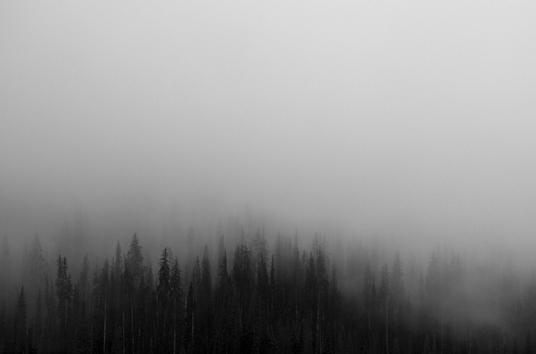
\includegraphics{images/jungle.jpg}
\end{center}
\end{document}
